\subsection{大原型机测试}

对于大原型机的测试主要分为两个部分,一部分是气体系统以及Slow control系统的测试,另一部分为电子学测试以及数据分析。气体系统和Slow Control的工作主要由BNL的人员完成,在此不多做介绍。笔者主要参与的为电子学测试和数据分析工作。将在下文当中进行详细介绍。

和小原型机测试一样,首先需要解决的是电子学通道和实际读出条对应的map问题。因为在最终的探测器丝室的设计中读出条在同一个方向上被分成多段,所以大原型机也进行了类似的设计,在同一个方向上读出条被分成多段,这使得map工作相对于小原型机变得复杂了一些。大原型机的读出条和插口对应如图\ref{fig:LargePrototype_PCB}所示。在实际的原型机测试当中为了测试读出条分段对ghost hit的排除能力,要让左图右下角即读出条分段最多的部分相互重叠,这就要求一个室的布局应该是另一个室沿着左上到右下的对角线镜像反转。左图和右图分别为两个室的布局,其中右图为左图沿对角线反转后得到,和实际的原型机读出条分布相符。
这样就导致的读出条的编号方式需要进行改变,在小原型机当中读出条只有一列读出条,只需按照顺序编号即可,当有多行strip之后单纯按顺序编号会导致读出条编号混乱,无法直接使用小原型机的map文件,所以map需要重新编写。对于单个前端电子学板的通道和读出条对应的部分还是和图\ref{fig:TPX_map}所示相同,但读出条的编号发生了改变,编号从单纯的$n_{strip}$变成了($n_{row} * 1000 + n_{strip}$)。整个编号的最高位为行号。插口号和读出条行号的对应关系见表\ref{tab:LargePrototype_map}。对于另一个室来说,因为发生了镜像翻转,FEE上的通道和读出条对应的关系也发生了翻转,需要在map的头文件里额外的添加函数来进行翻转。
\begin{table}[h!]
    \centering
    \caption{大原型机插口号和读出条行号对应关系}
    \label{tab:LargePrototype_map}
    \begin{tabularx}{1\textwidth} {| >{\centering\arraybackslash}X |>{\centering\arraybackslash}X |>{\centering\arraybackslash}X |>{\centering\arraybackslash}X |}
        \hline
        行号 & 1 & 2 & 3 \\
        \hline
        插口号& 1 4 7 & 2 5 8 10 12 14 & 3 6 9 11 13 15 \\
        \hline
    \end{tabularx}
\end{table}

\begin{figure}[htb]
    \begin{center}
    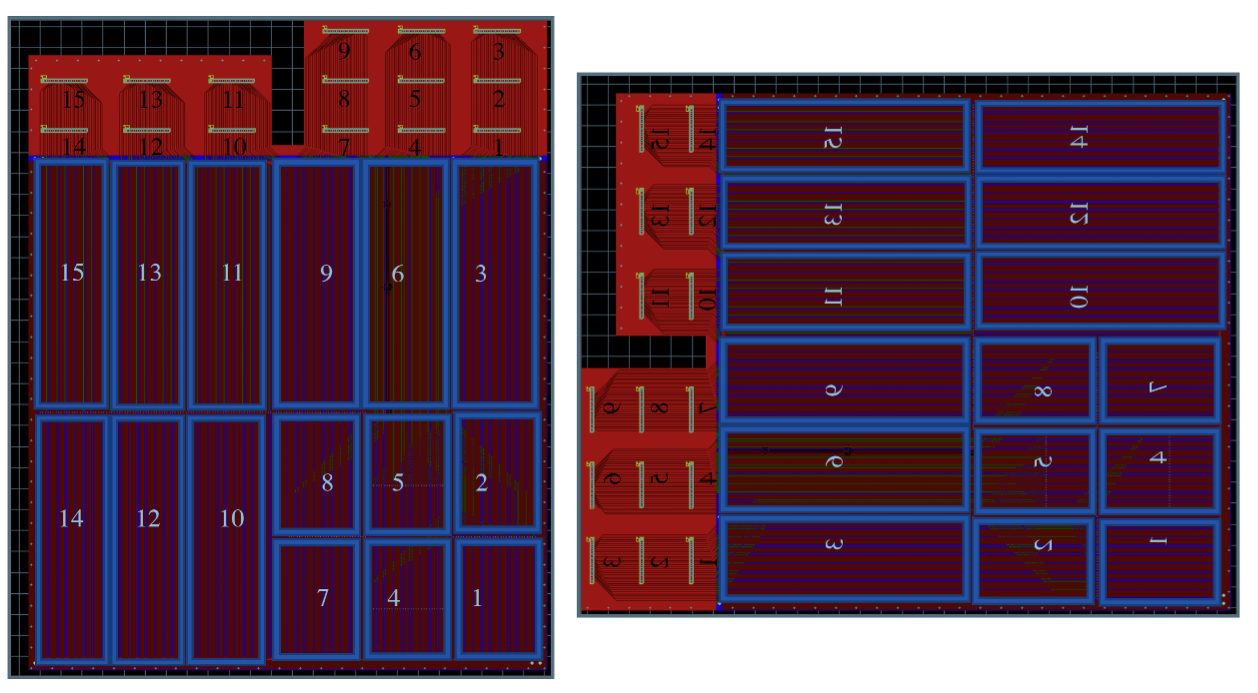
\includegraphics[width=0.8\textwidth,clip]{figures/Chapter3/LargePrototype_PCB.png}
    \end{center}
    \caption[sTGC 大原型机Strip示意图]{sTGC 大原型机Strip示意图白色数字标明了不同的插口对应的strip区域,例如当前端电子学卡插在编号为1的slot上时将会和编号为1的读出条区域相连接。左图和右图分别为大原型机两个不同室的读出条分布。}
    \label{fig:LargePrototype_PCB}
\end{figure}

同时因为大原型机的前端电子学插口是为了TPX电子学所设计的,而最终sTGC使用的电子学是VMM芯片,并不能直接连接到大原型机的电子学插口上面去,需要一个转接器来让VMM电子学可以插到TPX电子学对应的插口上面去。这就使得当使用VMM电子学进行测试的时候,map的头文件里需要额外添加一个关于VMM电子学通道和TPX电子学通道对应的函数。

